\chapter{Descripción de los biopotenciales} 
%//////////////////////////////////////////////////////////////////////////////////////////////////////
\section{Características de la señal}
%//////////////////////////////////////////////////////////////////////////////////////////////////////
Las señales de electromografía se encuentran en un rango de frecuencias que varia desde los 25 $Hz$ hasta varios $kHz$, con amplitudes que varia entre los 100 $\mu V$ y los 90 $mV$ dependiendo del tipo de señal y los electrodos utilizados \cite{webster2009medical}, figura \ref{voltaje_vs_frecuencia}. \\

Al emplear electrodos de montaje superficial el nivel de las señales es generalmente bajo con amplitudes pico que van desde los 0.1 a 1 $mV$, la impedancia es usualmente baja variando entre 200 a 5000 $\Omega$ lo cual a su vez depende del tipo de electrodo, la interfaz electrodo electrolito y la frecuencia a la que se determino la impedancia \cite{webster2009medical}.

Una ventaja de que solo se presenten bajas frecuencias en la señal es que pueden ser filtradas mas fácilmente \cite{webster2009medical}.

\begin{figure}[H]
  \centering
  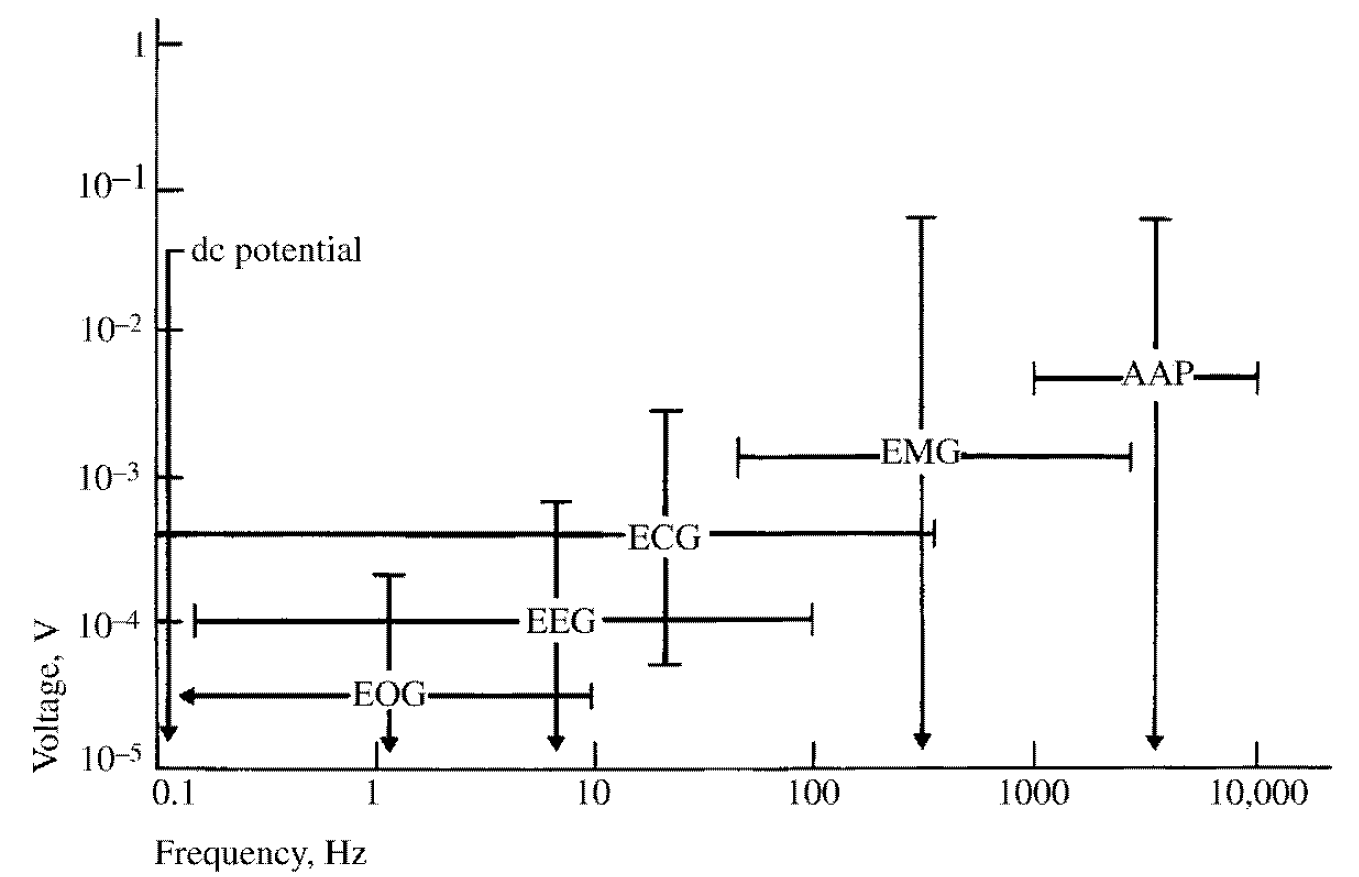
\includegraphics[width=0.8\textwidth]{Capitulo_1/voltaje_vs_frecuencia.png}
  \caption{Rangos de frecuencia y voltaje de algunas señales de biopotencial, EOC (Electrooculograma), EEG (Electroenfalograma), ECG (Electrocardiograma), EMG (Electromiograma), AAP (Potencial de acción de los axones) \cite{webster2009medical}.}
  \label{voltaje_vs_frecuencia} 
\end{figure}
%//////////////////////////////////////////////////////////////////////////////////////////////////////
\section{Medición de la impedancia}
%//////////////////////////////////////////////////////////////////////////////////////////////////////
Al emplear electrodos superficiales en la piel, al momento de realizar las mediciones de los biopotenciales debe considerarse dos interfaces, la presente entre el electrodo y el electrolito y la que representa la piel, para mostrar el nivel de complejidad que trae incluir el efecto de la piel en el modelo en la figura \ref{Imagen piel} se puede ver un diagrama seccional de un bloque magnificado de piel.

\begin{figure}[H]
  \centering
  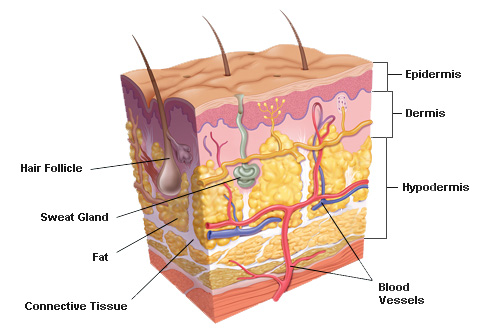
\includegraphics[width=0.6\textwidth]{Capitulo_1/skindiagram.jpg}
  \caption{Sección amplificada de un bloque de piel onde se puede apreciar las multiples capas que presenta la misma \cite{iskin2015}.}
  \label{Imagen piel} 
\end{figure}



\begin{figure}[H]
  \centering
  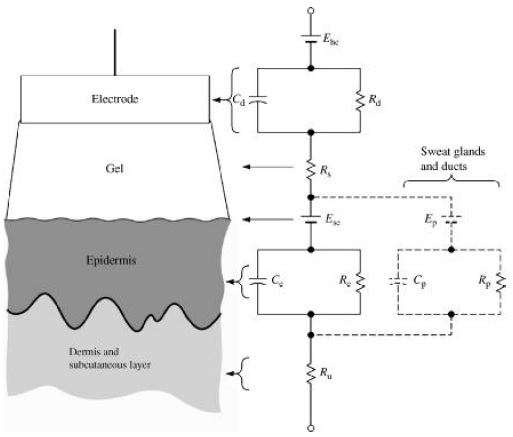
\includegraphics[width=0.6\textwidth]{Capitulo_1/skindiagramcircuit.jpg}
  \caption{Circuito electrico equivalente de un electrodo sobre la piel \cite{webster2009medical}.}
  \label{circuito equivalente} 
\end{figure}

% La tabla que se presenta a continuación se obtuvo de 
% https://hermanwallace.com/download/The_ABC_of_EMG_by_Peter_Konrad.pdf

Los resultados obtenidos por medio de las pruebas deben encontrarse dentro de los siguientes rangos para asegurar el apropiado funcionamiento del electromiógrafo \cite{konrad2005abc}.

\begin{table}[H]
\centering
\caption{ Recomendaciones para los rangos de impedancia electrodo/piel \cite{konrad2005abc}}
\label{Rango impedancias}
\begin{tabular}{ll}
\hline
\multicolumn{1}{c}{\textbf{Rango de impedancias}}        & \multicolumn{1}{c}{\textbf{Recomendaciones}} \\ 
\multicolumn{1}{c}{\textbf{$k\Omega$}}                   &   \\ 
\hline \hline
1-5   & Muy buena condición  \\
5-10  & Bueno y recomendado si es factible \\
10-30 & Aceptable para condiciones fáciles \\
30-50 & Menos bueno, se necesita atención \\
$>50$ & Debe evitarse o requiere un segundo ciclo de limpieza \\
\hline
\end{tabular}
\end{table}

En el laboratorio se encuentra disponible un generador de funciones Tektronix CFG253 el cual posee una impedancia interna ($R_{fg}$) de 50 $\Omega$ donde de acuerdo al principio de máxima potencia se llego a la conclusión que la máxima corriente que puede generar es de 400 $mApp$.

\begin{align}\label{eq:eq2}
i_o=\frac{V_{max}}{R_{fg}}=\frac{10 Vpp}{50 \Omega}=400 mA
\end{align}

Su frecuencia de trabajo varia desde los 0.2 $Hz$ a los 2 $MHz$; con respecto a la amplitud y acorde con el manual de usuario, el osciloscopio empleado en las prácticas de laboratorio tiene dos rangos de trabajo:
      \begin{itemize}
      \item 0-20 Vpp (Voltios pico a pico).
        \begin{itemize}
          \item100 mv a 20 Vpp (circuito abierto)
          \item50 mv a 10 Vpp (Carga de 50 $\Omega$)
        \end{itemize}    
      \item 0-2 Vpp
        \begin{itemize}
          \item 10 mv a 2 Vpp (circuito abierto)
          \item 5 mv a 1 Vpp (Carga de 50 $\Omega$)
        \end{itemize}
      \end{itemize}   

% Tambien se debe incluir esto
% https://www.tuv.com/media/usa/aboutus_1/pressreleases/fieldevaluation/Effects_of_Electrical_Current_in_Human_Body.pdf

La interface presente entre las señales producidas por los músculos presenta una porción resistiva y una porción reactiva capacitiva tal y como se mencionó antes, sin embargo se verifica al observar la reducción de la corriente al ser aplicada una fem alterna y su incremento a medida que la frecuencia va aumentando comportamiento característico de un condensador, además de que en las gráficas obtenidas en el osciloscopio la corriente se encuentra adelantada con respecto al voltaje.

\begin{table}[H]
\centering
\caption{My caption}
\label{my-label}
\begin{tabular}{lllllllll}
\hline
 & \multicolumn{4}{c}{Sujeto 1} & \multicolumn{4}{c}{Sujeto 2} \\
\hline
\multicolumn{1}{c}{f} & \multicolumn{1}{c}{v} & \multicolumn{1}{c}{i} & \multicolumn{1}{c}{pha} & \multicolumn{1}{c}{r} & \multicolumn{1}{c}{v} & \multicolumn{1}{c}{i} & \multicolumn{1}{c}{pha} & \multicolumn{1}{c}{r} \\
\multicolumn{1}{c}{$Hz$} & \multicolumn{1}{c}{$V$} & \multicolumn{1}{c}{$mA$} & \multicolumn{1}{c}{$^\circ$} & \multicolumn{1}{c}{$k\Omega$} & \multicolumn{1}{c}{$V$} & \multicolumn{1}{c}{$mA$} & \multicolumn{1}{c}{$^\circ$} & \multicolumn{1}{c}{$k\Omega$} \\
\hline
\hline
10	&	16.80	&	0.40	&	-71.96	&	13.01	&	16.80	&	0.64	&	-65.01	&	11.09	\\
100	&	20.40	&	1.88	&	-68.80	&	3.92	&	20.20	&	2.92	&	-61.50	&	3.30	\\
500	&	20.40	&	6.80	&	-60.10	&	1.50	&	20.00	&	10.00	&	-51.00	&	1.26	\\
600	&	20.20	&	7.68	&	-58.30	&	1.38	&	20.20	&	11.20	&	-45.70	&	1.26	\\
800	&	20.00	&	9.80	&	-51.70	&	1.26	&	19.80	&	13.00	&	-40.90	&	1.15	\\
900	&	20.00	&	10.60	&	-51.56	&	1.17	&	19.60	&	13.80	&	-39.50	&	1.10	\\
1000	&	20.00	&	11.20	&	-50.70	&	1.13	&	19.60	&	14.20	&	-37.50	&	1.10	\\
1500	&	19.60	&	13.60	&	-41.00	&	1.09	&	19.60	&	16.00	&	-28.50	&	1.08	\\
2000	&	19.80	&	15.40	&	-36.70	&	1.03	&	19.60	&	17.20	&	-25.10	&	1.03	\\
3000	&	20.00	&	17.40	&	-30.60	&	0.99	&	19.60	&	18.40	&	-19.40	&	1.00	\\
5000	&	19.60	&	19.60	&	-23.70	&	0.92	&	19.40	&	20.20	&	-17.20	&	0.92	\\
\hline
\end{tabular}
\end{table}
%//////////////////////////////////////////////////////////////////////////////////////////////////////
\section{Magnitud de la señal de salida y factor de amplificación requerido}
%//////////////////////////////////////////////////////////////////////////////////////////////////////
Para caracterizar la señal de entrada se propuso el montaje que se muestra en la figura \ref{fig:esquematico}. El circuito mostrado presenta una ganancia de tensión $A_v = 500$; las entradas $V_1$ y $V_2$ corresponden a la entrada diferencial provenientes de los electrodos, junto con el de referencia que viene dad por la conexión a tierra del circuito .

\begin{figure}[H]
\centering
\begin{subfigure}{.4\textwidth}
  \centering
  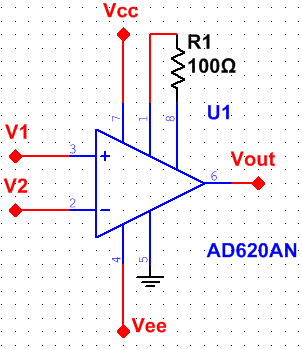
\includegraphics[width=.8\linewidth]{Capitulo_1/Esquematico.png}
  \caption{Esquematico}
  \label{fig:esquematico}
\end{subfigure}
\begin{subfigure}{.4\textwidth}
  \centering
  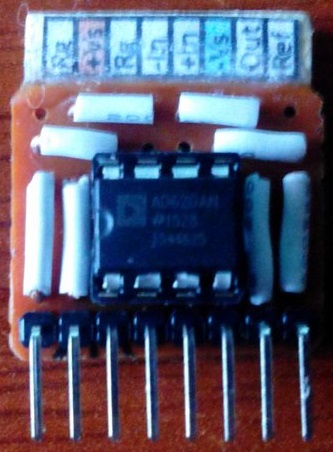
\includegraphics[width=.8\linewidth]{Capitulo_1/placa.jpg}
  \caption{Placa de pruebas}
  \label{fig:placa}
\end{subfigure}
\caption{Esquema del circuito empleado.}
\label{fig:esquema}
\end{figure}

Para realizar la caracterización de la señal de entrada de los músculos, se realizó mediante un amplificador de instrumentación (AD620), en el cual se diseñó el diseño para obtener una ganancia de 500, con el fin de lograr observar las señales producidas por los músculos que se estaban obteniendo por los electrodos. Primero mediante el generador de señales se logró corroborar el funcionamiento y la ganancia esperada. Posteriormente se realizaron pruebas con la señal de los músculos y se obtuvo la siguiente respuesta dada en la figura \ref{fig:resopamp}.

cabe recalcar que si el maximo pico fue obtenido a 7.4 $V$ entonces la señal que lo produjo tuvo una magnitud de 14.8 $mV$. 

\begin{figure}[H]
  \centering
  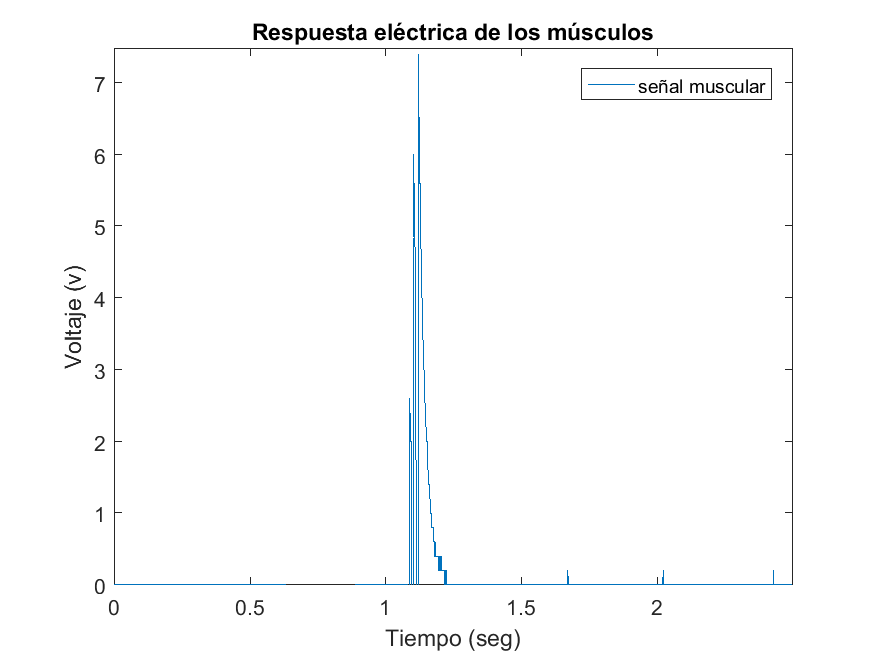
\includegraphics[width=1\textwidth]{Capitulo_1/resultadoopamp.png}
  \caption{Repuesta obtenida con el amplificador de instrumentación.}
  \label{fig:resopamp} 
\end{figure}

\subsection{Algunas Observaciones al Respecto}

Durante el desarrollo de la práctica se evidenciaron algunos aspectos que son necesarios tener en cuenta.

\begin{enumerate}
\item Se utilizó un circuito integrado para caracterizar la señal de entrada del brazo con el objetivo de tener una referencia en términos de desempeño para el montaje discreto que se debe emplear en el montaje final.
\item Para obtener la señal mostrada en la figura \ref{fig:resopamp} fue necesario utilizar además de los electrodos mismos, unas correas que garantizaran que hubiese contacto entre el electrodo y el cable que va hacia las entradas del amplificador. 
\end{enumerate}
%http://www.analog.com/media/en/technical-documentation/data-sheets/AD620.pdf

%http://bioinstrumentacion.eia.edu.co/WebEstudiantes/2005I/EMG/materialesymetodos.htm


